\documentclass[12pt]{article}
\usepackage{amsmath}
\usepackage{amssymb}
\usepackage{amsthm}
\usepackage{geometry}
\usepackage[utf8]{inputenc}
\usepackage{hyperref}
\usepackage{tikz}

% TikZ libraries needed for diagrams
\usetikzlibrary{intersections, calc, shapes.geometric}

\geometry{
 a4paper,
 total={170mm,257mm},
 left=20mm,
 top=20mm,
}

\newtheorem{theorem}{Theorem}
\newtheorem*{solution}{Solution}

\author{Vu Hung Nguyen}
\title{Pappus's hexagon theorem}
\date{}

\begin{document}

\maketitle

\section{Overview}

This document presents Pappus's hexagon theorem, one of the fundamental results in projective geometry. We explore its statement, historical context, and provide proofs using both affine transformations and the elegant connection to Pascal's Theorem. The document is designed for olympiad-level high school students and advanced mathematics enthusiasts who wish to understand this beautiful geometric result and its deep connections to projective geometry.

I was introduced to Pappus's theorem when I was in year 9. At that time, of course, I was not able to prove it, but I understood the concepts of affine transformations and ideas about higher linear transformations. It is a beautiful and inspiring theorem. The theorem is niche, but it may be helpful for olympiad problems, hopefully.

\section{Problem Statements}

\subsection{Pappus's hexagon theorem}

\begin{theorem}[Pappus's hexagon theorem]
Let $A, B, C$ be three distinct points on a line $g$, and let $a, b, c$ be three distinct points on another line $h$.

Consider the intersection points:
\begin{align*}
    X &= (Ab) \cap (aB) \\
    Y &= (Ac) \cap (aC) \\
    Z &= (Bc) \cap (bC)
\end{align*}

Then the points $X, Y, \text{ and } Z$ are collinear. This common line is called the \textbf{Pappus line}.
\end{theorem}

\begin{figure}[h!]
    \centering
    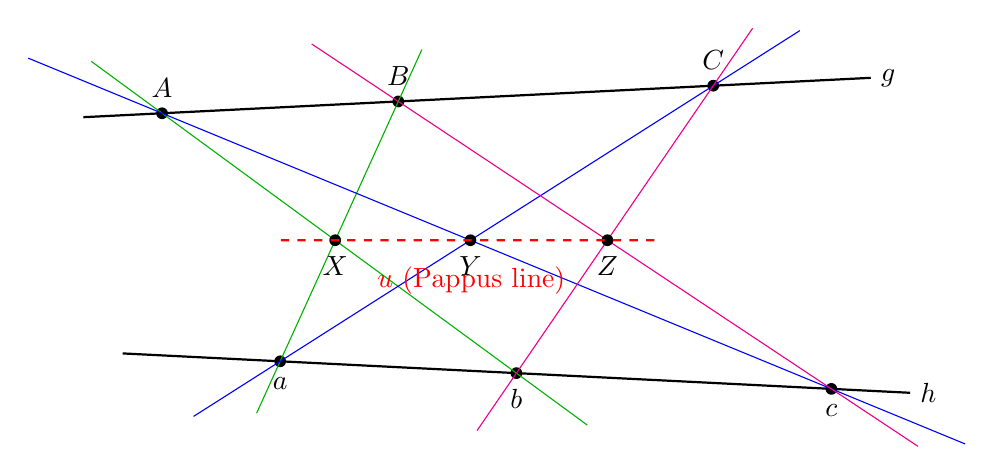
\begin{tikzpicture}[
        point/.style={circle, fill, inner sep=1.5pt}
    ]
        
        % Define coordinates for lines g and h (non-parallel)
        \coordinate (g1) at (0, 3);
        \coordinate (g2) at (10, 3.5);
        \coordinate (h1) at (0.5, 0);
        \coordinate (h2) at (10.5, -0.5);

        % Draw lines g and h
        \draw[thick, name path=g] (g1) -- (g2) node[right] {$g$};
        \draw[thick, name path=h] (h1) -- (h2) node[right] {$h$};

        % Place points A, B, C on line g and a, b, c on line h
        \node[point, label=above:$A$] (A) at ($(g1)!0.1!(g2)$) {};
        \node[point, label=above:$B$] (B) at ($(g1)!0.4!(g2)$) {};
        \node[point, label=above:$C$] (C) at ($(g1)!0.8!(g2)$) {};
        
        \node[point, label=below:$a$] (a) at ($(h1)!0.2!(h2)$) {};
        \node[point, label=below:$b$] (b) at ($(h1)!0.5!(h2)$) {};
        \node[point, label=below:$c$] (c) at ($(h1)!0.9!(h2)$) {};

        % Draw the intersecting lines
        % Lines for X (Green)
        \draw[green!70!black, name path=Ab] ($(A)!-0.2!(b)$) -- ($(A)!1.2!(b)$);
        \draw[green!70!black, name path=aB] ($(a)!-0.2!(B)$) -- ($(a)!1.2!(B)$);

        % Lines for Y (Blue)
        \draw[blue, name path=Ac] ($(A)!-0.2!(c)$) -- ($(A)!1.2!(c)$);
        \draw[blue, name path=aC] ($(a)!-0.2!(C)$) -- ($(a)!1.2!(C)$);

        % Lines for Z (Magenta)
        \draw[magenta, name path=Bc] ($(B)!-0.2!(c)$) -- ($(B)!1.2!(c)$);
        \draw[magenta, name path=bC] ($(b)!-0.2!(C)$) -- ($(b)!1.2!(C)$);
        
        % Find the intersections
        \path[name intersections={of=Ab and aB, by=X}];
        \path[name intersections={of=Ac and aC, by=Y}];
        \path[name intersections={of=Bc and bC, by=Z}];

        % Draw and label the intersection points
        \node[point, label=below:$X$] at (X) {};
        \node[point, label=below:$Y$] at (Y) {};
        \node[point, label=below:$Z$] at (Z) {};

        % Draw the Pappus line (u)
        \draw[red, dashed, thick] ($(X)!-0.2!(Z)$) -- ($(X)!1.2!(Z)$) 
            node[midway, below, yshift=-2mm] {$u$ (Pappus line)};

    \end{tikzpicture}
    \caption{A diagram illustrating Pappus's hexagon theorem.}
\end{figure}

\subsection{Special Case: Parallel Lines}

When the lines $g$ and $h$ are parallel, Pappus's hexagon theorem still holds. In this case, the two lines never intersect, but the theorem remains valid in the affine plane. The Pappus line $u$ will be parallel to both $g$ and $h$ in this configuration.

\begin{figure}[h!]
    \centering
    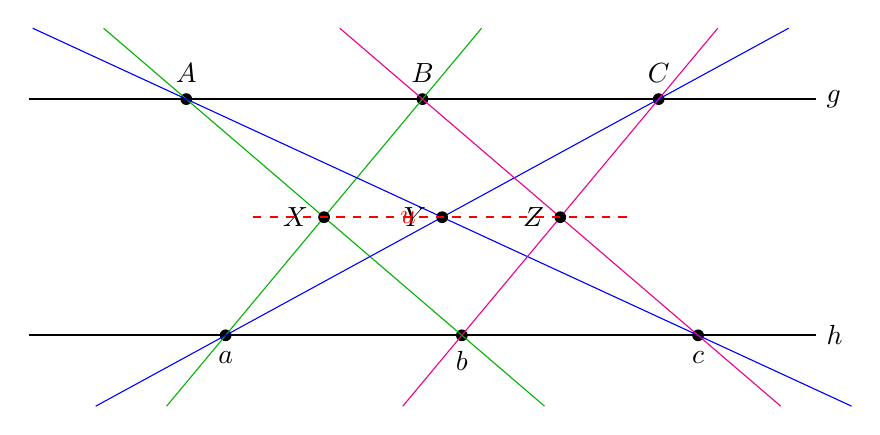
\begin{tikzpicture}[
        point/.style={circle, fill, inner sep=1.5pt}
    ]
        
        % Define coordinates for parallel lines g and h
        \coordinate (g1) at (0, 3);
        \coordinate (g2) at (10, 3);
        \coordinate (h1) at (0, 0);
        \coordinate (h2) at (10, 0);

        % Draw parallel lines g and h
        \draw[thick, name path=g] (g1) -- (g2) node[right] {$g$};
        \draw[thick, name path=h] (h1) -- (h2) node[right] {$h$};

        % Place points A, B, C on line g and a, b, c on line h
        \node[point, label=above:$A$] (A) at (2, 3) {};
        \node[point, label=above:$B$] (B) at (5, 3) {};
        \node[point, label=above:$C$] (C) at (8, 3) {};
        
        \node[point, label=below:$a$] (a) at (2.5, 0) {};
        \node[point, label=below:$b$] (b) at (5.5, 0) {};
        \node[point, label=below:$c$] (c) at (8.5, 0) {};

        % Draw the intersecting lines
        \draw[green!70!black, name path=Ab] ($(A)!-0.3!(b)$) -- ($(A)!1.3!(b)$);
        \draw[green!70!black, name path=aB] ($(a)!-0.3!(B)$) -- ($(a)!1.3!(B)$);

        \draw[blue, name path=Ac] ($(A)!-0.3!(c)$) -- ($(A)!1.3!(c)$);
        \draw[blue, name path=aC] ($(a)!-0.3!(C)$) -- ($(a)!1.3!(C)$);

        \draw[magenta, name path=Bc] ($(B)!-0.3!(c)$) -- ($(B)!1.3!(c)$);
        \draw[magenta, name path=bC] ($(b)!-0.3!(C)$) -- ($(b)!1.3!(C)$);
        
        % Find the intersections
        \path[name intersections={of=Ab and aB, by=X}];
        \path[name intersections={of=Ac and aC, by=Y}];
        \path[name intersections={of=Bc and bC, by=Z}];

        % Draw and label the intersection points
        \node[point, label=left:$X$] at (X) {};
        \node[point, label=left:$Y$] at (Y) {};
        \node[point, label=left:$Z$] at (Z) {};

        % Draw the Pappus line (u) - parallel to g and h
        \draw[red, dashed, thick] ($(X)!-0.3!(Z)$) -- ($(X)!1.3!(Z)$) 
            node[midway, left, xshift=-2mm] {$u$};

    \end{tikzpicture}
    \caption{Pappus's hexagon theorem when lines $g$ and $h$ are parallel.}
\end{figure}

\subsection{Special Case: Perpendicular Lines}

When the lines $g$ and $h$ are perpendicular, Pappus's hexagon theorem provides a particularly elegant configuration. The perpendicular case can be transformed to the coordinate axes, making calculations more straightforward.

\begin{figure}[h!]
    \centering
    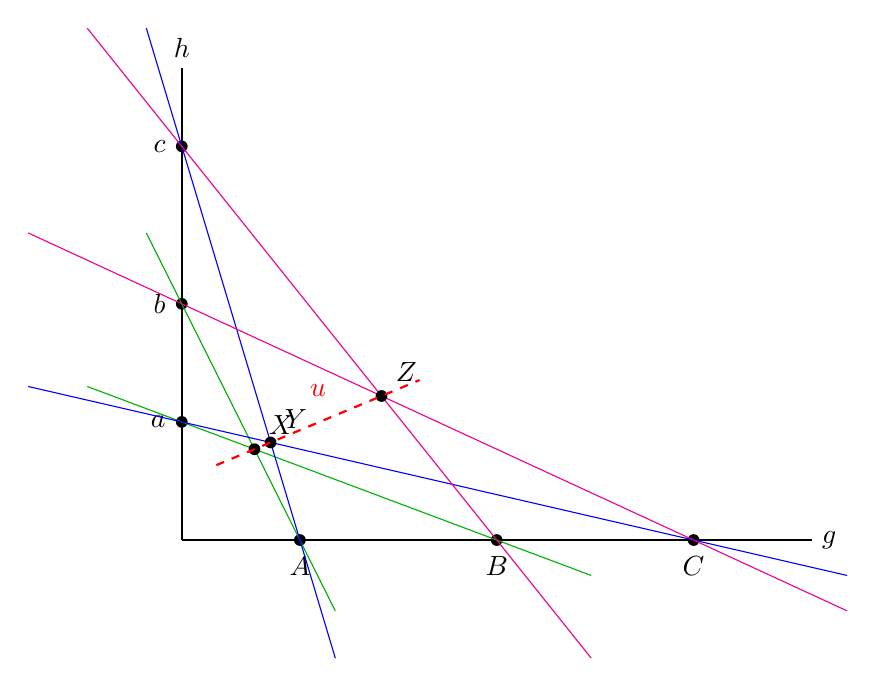
\begin{tikzpicture}[
        point/.style={circle, fill, inner sep=1.5pt}
    ]
        
        % Define coordinates for perpendicular lines g and h
        \coordinate (g1) at (0, 0);
        \coordinate (g2) at (8, 0);
        \coordinate (h1) at (0, 0);
        \coordinate (h2) at (0, 6);

        % Draw perpendicular lines g (horizontal) and h (vertical)
        \draw[thick, name path=g] (g1) -- (g2) node[right] {$g$};
        \draw[thick, name path=h] (h1) -- (h2) node[above] {$h$};

        % Place points A, B, C on line g (x-axis) and a, b, c on line h (y-axis)
        \node[point, label=below:$A$] (A) at (1.5, 0) {};
        \node[point, label=below:$B$] (B) at (4, 0) {};
        \node[point, label=below:$C$] (C) at (6.5, 0) {};
        
        \node[point, label=left:$a$] (a) at (0, 1.5) {};
        \node[point, label=left:$b$] (b) at (0, 3) {};
        \node[point, label=left:$c$] (c) at (0, 5) {};

        % Draw the intersecting lines
        \draw[green!70!black, name path=Ab] ($(A)!-0.3!(b)$) -- ($(A)!1.3!(b)$);
        \draw[green!70!black, name path=aB] ($(a)!-0.3!(B)$) -- ($(a)!1.3!(B)$);

        \draw[blue, name path=Ac] ($(A)!-0.3!(c)$) -- ($(A)!1.3!(c)$);
        \draw[blue, name path=aC] ($(a)!-0.3!(C)$) -- ($(a)!1.3!(C)$);

        \draw[magenta, name path=Bc] ($(B)!-0.3!(c)$) -- ($(B)!1.3!(c)$);
        \draw[magenta, name path=bC] ($(b)!-0.3!(C)$) -- ($(b)!1.3!(C)$);
        
        % Find the intersections
        \path[name intersections={of=Ab and aB, by=X}];
        \path[name intersections={of=Ac and aC, by=Y}];
        \path[name intersections={of=Bc and bC, by=Z}];

        % Draw and label the intersection points
        \node[point, label=above right:$X$] at (X) {};
        \node[point, label=above right:$Y$] at (Y) {};
        \node[point, label=above right:$Z$] at (Z) {};

        % Draw the Pappus line (u)
        \draw[red, dashed, thick] ($(X)!-0.3!(Z)$) -- ($(X)!1.3!(Z)$) 
            node[midway, above, yshift=2mm] {$u$};

    \end{tikzpicture}
    \caption{Pappus's hexagon theorem when lines $g$ and $h$ are perpendicular.}
\end{figure}

\section{History of Pappus's hexagon theorem and Pappus}

Pappus of Alexandria (c. 290--350 CE) was one of the last great mathematicians of antiquity. He lived in Alexandria, Egypt, during the later period of the Roman Empire. Pappus is best known for his work \textit{Collection} (or \textit{Synagoge}), a comprehensive compilation of Greek mathematical knowledge that preserved many results that would otherwise have been lost.

Pappus's hexagon theorem is one of the fundamental results in projective geometry. It was stated by Pappus in his \textit{Collection}, though the modern formulation and proof techniques have evolved significantly since then.

The theorem holds a special place in the history of mathematics because:
\begin{itemize}
    \item It is one of the earliest results in what we now call projective geometry
    \item It demonstrates the power of projective methods in solving geometric problems
    \item It connects to deeper results like Pascal's Theorem, showing the unity of geometric theory
    \item It remains a cornerstone result in modern algebraic geometry
\end{itemize}

Pappus's work influenced many later mathematicians, including Desargues, Pascal, and the founders of modern projective geometry in the 19th century.

\section{Required Knowledge to Read This Document}

Before diving into the solutions, readers should be familiar with the following concepts:

\subsection{Linear Algebra}
Basic understanding of vectors, linear transformations, and coordinate systems. Knowledge of matrix operations and their geometric interpretations will be helpful.

\subsection{Linear Transformations}
A linear transformation $T: \mathbb{R}^2 \to \mathbb{R}^2$ preserves the origin and satisfies $T(\alpha \mathbf{v} + \beta \mathbf{w}) = \alpha T(\mathbf{v}) + \beta T(\mathbf{w})$ for all vectors $\mathbf{v}, \mathbf{w}$ and scalars $\alpha, \beta$. Linear transformations include rotations, reflections, scaling, and shearing.

\subsection{Affine Transformations}
An \textbf{affine transformation} is a composition of a linear transformation and a translation. Formally, $T(\mathbf{x}) = A\mathbf{x} + \mathbf{b}$ where $A$ is a matrix and $\mathbf{b}$ is a vector. Affine transformations preserve:
\begin{itemize}
    \item Collinearity (points on a line remain on a line)
    \item Parallelism (parallel lines remain parallel)
    \item Ratios of distances along parallel lines
\end{itemize}

The key property we use is that affine transformations preserve collinearity, which allows us to simplify geometric problems by transforming them to more convenient coordinate systems.

\subsection{Projective Geometry}
Projective geometry extends Euclidean geometry by adding ``points at infinity'' and treating parallel lines as meeting at infinity. This unification allows many theorems to be stated more elegantly. The projective plane can be thought of as the Euclidean plane plus a ``line at infinity.''

In projective geometry, conic sections (circles, ellipses, parabolas, hyperbolas) are unified, and degenerate cases like two intersecting lines are also considered conics. This perspective is crucial for understanding the connection between Pappus's hexagon theorem and Pascal's Theorem.

\section{Solutions}

We present two approaches to proving Pappus's hexagon theorem: one using affine transformations (more computational) and one using Pascal's Theorem (more elegant and conceptual).

\noindent\textbf{Note:} Additional proofs of Pappus's hexagon theorem, including coordinate geometry proofs and other approaches, can be found on Wikipedia: \href{https://en.wikipedia.org/wiki/Pappus\%27s_hexagon_theorem}{https://en.wikipedia.org/wiki/Pappus's hexagon theorem}.

\subsection{Proof Using Affine Transformations}

The strategy is to use an affine transformation to simplify the problem, then verify the result in the simplified case. Since affine transformations preserve collinearity, the result will hold in the general case.

\subsubsection{The Big Idea}

An affine transformation can ``warp'' the plane through translations, rotations, scaling, and shearing, but it preserves the property we care about: collinearity. If three points are collinear before transformation, they remain collinear after.

\subsubsection{Case 1: Intersecting Lines}

We consider the case where lines $g$ and $h$ intersect. By applying an affine transformation, we can map:
\begin{itemize}
    \item Line $g$ to the $x$-axis ($y = 0$)
    \item Line $h$ to the $y$-axis ($x = 0$)
    \item The intersection point to the origin $(0,0)$
\end{itemize}

After this transformation, we have:
\begin{itemize}
    \item Points $A, B, C$ on the $x$-axis: $A = (A_x, 0)$, $B = (B_x, 0)$, $C = (C_x, 0)$
    \item Points $a, b, c$ on the $y$-axis: $a = (0, a_y)$, $b = (0, b_y)$, $c = (0, c_y)$
\end{itemize}

Using the intercept form of a line ($\frac{x}{x_{\text{int}}} + \frac{y}{y_{\text{int}}} = 1$), we can write equations for the lines:
\begin{itemize}
    \item Line $Ab$: $\frac{x}{A_x} + \frac{y}{b_y} = 1$
    \item Line $aB$: $\frac{x}{B_x} + \frac{y}{a_y} = 1$
\end{itemize}

Solving these systems for each intersection point $X, Y, Z$ and then verifying that they are collinear (by checking that the slopes $m_{XY} = m_{XZ}$) completes the proof. The algebra is tedious but straightforward, and the key insight is that the slopes turn out to be identical.

\subsubsection{Case 2: Parallel Lines}

When $g$ and $h$ are parallel, we can transform them to horizontal lines $y = 0$ and $y = 1$. A similar coordinate geometry argument shows that $X, Y, Z$ are collinear, with the Pappus line being parallel to $g$ and $h$.

\begin{solution}[Affine Transformation Proof]
By applying an affine transformation, we reduce the general case to a coordinate geometry problem. In the simplified coordinate system (axes or parallel lines), direct calculation shows that the three intersection points $X, Y, Z$ have the same slope, hence are collinear. Since affine transformations preserve collinearity, the result holds in the original configuration.
\end{solution}

\subsection{Proof Using Pascal's Theorem}

A more elegant proof recognizes that Pappus's hexagon theorem is a special case of Pascal's Theorem. This connection reveals the deeper structure of projective geometry.

\subsubsection{The Connection}

We view the two lines $g$ and $h$ as a \textbf{degenerate conic}---a conic section that has ``degenerated'' into two lines. In projective geometry, a pair of intersecting lines is considered a degenerate conic, defined by the equation $(ax + by + c)(dx + ey + f) = 0$.

\subsubsection{Constructing the Hexagon}

We form a hexagon by alternating points from the two lines: $A-b-C-a-B-c$. This hexagon is inscribed in our degenerate conic (since all six vertices lie on $g \cup h$).

\subsubsection{Applying Pascal's Theorem}

Pascal's Theorem (discussed in detail in the next section) states that for any hexagon inscribed in a conic, the three intersection points of opposite sides are collinear. For our hexagon $A-b-C-a-B-c$:
\begin{itemize}
    \item Opposite sides $(Ab)$ and $(aB)$ intersect at $X$
    \item Opposite sides $(bC)$ and $(Bc)$ intersect at $Z$
    \item Opposite sides $(Ca)$ and $(cA)$ intersect at $Y$
\end{itemize}

By Pascal's Theorem, $X, Y, Z$ are collinear---exactly the statement of Pappus's hexagon theorem!

\begin{solution}[Pascal's Theorem Proof]
Pappus's hexagon theorem follows immediately from Pascal's Theorem by recognizing that two lines form a degenerate conic. The hexagon $A-b-C-a-B-c$ inscribed in this degenerate conic has opposite sides intersecting at $X, Y, Z$, which must be collinear by Pascal's Theorem.
\end{solution}

\section{Pascal's Theorem}

\subsection{Statement of Pascal's Theorem}

\begin{theorem}[Pascal's Theorem]
Let $A, B, C, D, E, F$ be six distinct points on a conic section (ellipse, parabola, or hyperbola). Consider the hexagon $A-B-C-D-E-F$ inscribed in the conic. Let the three pairs of opposite sides intersect at:
\begin{align*}
    X &= (AB) \cap (DE) \\
    Y &= (BC) \cap (EF) \\
    Z &= (CD) \cap (FA)
\end{align*}
Then the points $X, Y, \text{ and } Z$ are collinear. This line is called the \textbf{Pascal line}.
\end{theorem}

\subsection{Note on Conic Sections}

A \textbf{conic section} is a curve obtained by intersecting a cone with a plane. The three main types are:
\begin{itemize}
    \item \textbf{Ellipse}: A closed curve (special case: circle)
    \item \textbf{Parabola}: An open curve with one branch
    \item \textbf{Hyperbola}: An open curve with two branches
\end{itemize}

In projective geometry, these are unified: all conics are projectively equivalent. 
Additionally, \textbf{degenerate conics}---pairs of lines (intersecting or parallel)---are also considered. 
This is why Pappus's hexagon theorem is a special case of Pascal's Theorem.

\subsection{Illustrations of Pascal's Theorem}

\begin{figure}[h!]
    \centering
    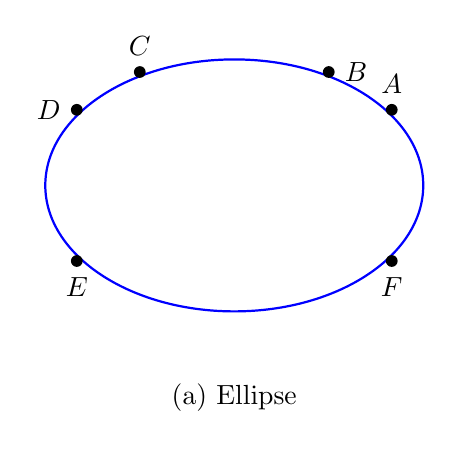
\begin{tikzpicture}[
        point/.style={circle, fill, inner sep=1.5pt},
        scale=0.8
    ]
        % Ellipse
        \draw[thick, blue] (0,0) ellipse (3cm and 2cm);
        
        % Points on ellipse
        \node[point, label=above:$A$] (A) at (2.5, 1.2) {};
        \node[point, label=right:$B$] (B) at (1.5, 1.8) {};
        \node[point, label=above:$C$] (C) at (-1.5, 1.8) {};
        \node[point, label=left:$D$] (D) at (-2.5, 1.2) {};
        \node[point, label=below:$E$] (E) at (-2.5, -1.2) {};
        \node[point, label=below:$F$] (F) at (2.5, -1.2) {};
        
        \node[below] at (0, -3) {(a) Ellipse};
    \end{tikzpicture}
    \hfill
    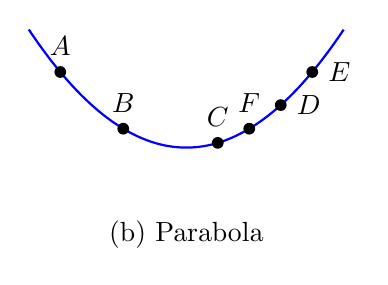
\begin{tikzpicture}[
        point/.style={circle, fill, inner sep=1.5pt},
        scale=0.8
    ]
        % Parabola: y = x^2/2 - 2, shifted and scaled
        \draw[thick, blue, domain=-2.5:2.5, samples=100] plot (\x, {0.3*\x*\x - 2});
        
        % Points on parabola
        \node[point, label=above:$A$] (A) at (-2, -0.8) {};
        \node[point, label=above:$B$] (B) at (-1, -1.7) {};
        \node[point, label=above:$C$] (C) at (0.5, -1.925) {};
        \node[point, label=right:$D$] (D) at (1.5, -1.325) {};
        \node[point, label=right:$E$] (E) at (2, -0.8) {};
        \node[point, label=above:$F$] (F) at (1, -1.7) {};
        
        \node[below] at (0, -3) {(b) Parabola};
    \end{tikzpicture}
    \hfill
    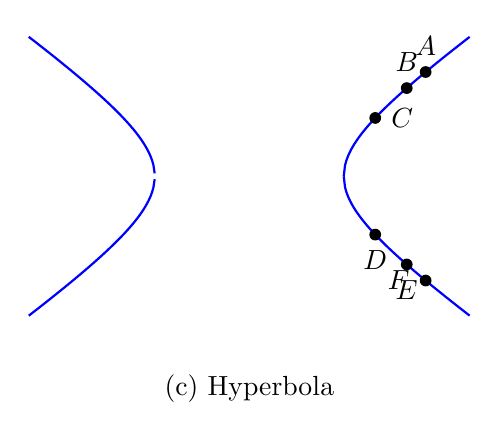
\begin{tikzpicture}[
        point/.style={circle, fill, inner sep=1.5pt},
        scale=0.8
    ]
        % Hyperbola: x^2/2.25 - y^2/1 = 1, so y = ±(1/1.5)*sqrt(x^2 - 2.25) for |x| >= 1.5
        % Using coefficient 0.7 for better visual scaling
        \draw[thick, blue, domain=1.5:3.5, samples=100] plot (\x, {0.7*sqrt(\x*\x - 2.25)});
        \draw[thick, blue, domain=1.5:3.5, samples=100] plot (\x, {-0.7*sqrt(\x*\x - 2.25)});
        \draw[thick, blue, domain=-3.5:-1.5, samples=100] plot (\x, {0.7*sqrt(\x*\x - 2.25)});
        \draw[thick, blue, domain=-3.5:-1.5, samples=100] plot (\x, {-0.7*sqrt(\x*\x - 2.25)});
        
        % Points on hyperbola (right branch) - calculated to lie exactly on the curve
        % For hyperbola y = ±0.7*sqrt(x^2 - 2.25), choosing x values and computing y
        \node[point, label=above:$A$] (A) at (2.8, {0.7*sqrt(2.8*2.8 - 2.25)}) {};
        \node[point, label=above:$B$] (B) at (2.5, {0.7*sqrt(2.5*2.5 - 2.25)}) {};
        \node[point, label=right:$C$] (C) at (2.0, {0.7*sqrt(2.0*2.0 - 2.25)}) {};
        \node[point, label=below:$D$] (D) at (2.0, {-0.7*sqrt(2.0*2.0 - 2.25)}) {};
        \node[point, label=below:$E$] (E) at (2.5, {-0.7*sqrt(2.5*2.5 - 2.25)}) {};
        \node[point, label=left:$F$] (F) at (2.8, {-0.7*sqrt(2.8*2.8 - 2.25)}) {};
        
        \node[below] at (0, -3) {(c) Hyperbola};
    \end{tikzpicture}
    \caption{Six points $A, B, C, D, E, F$ on (a) ellipse, (b) parabola, and (c) hyperbola.}
\end{figure}

\begin{figure}[htbp]
    \centering
    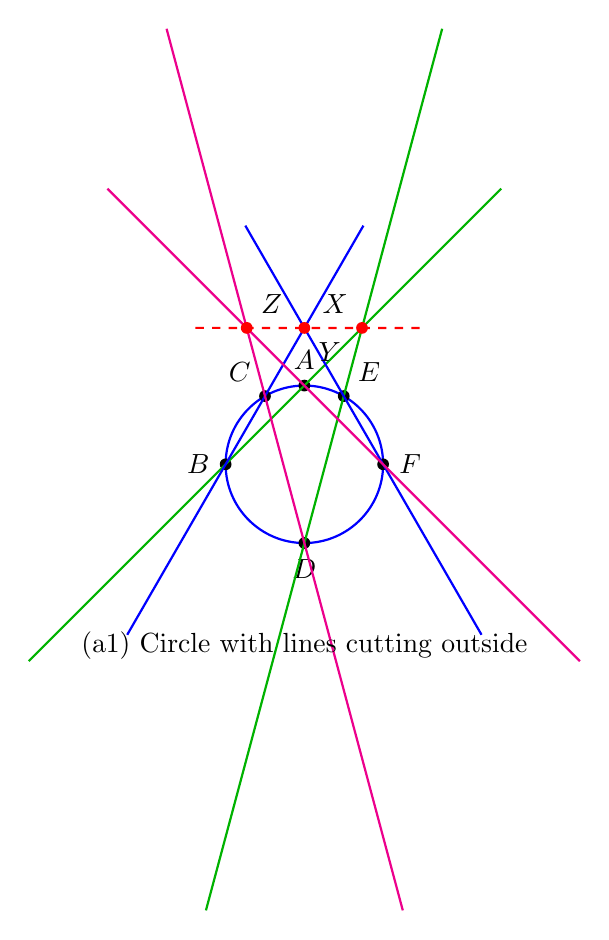
\begin{tikzpicture}[
        point/.style={circle, fill, inner sep=1.5pt},
        scale=1.0
    ]
        % Circle (unit circle)
        \draw[thick, blue] (0,0) circle (1cm);
        
        % Points on unit circle in order around circle: A -> B -> C -> D -> E -> F -> A
        % Hexagon order for Pascal's theorem: A-B-C-D-E-F
        % Using specified Cartesian coordinates on unit circle
        \node[point, label=above:$A$] (A) at (0, 1) {};   % 
        \node[point, label=left:$B$] (B) at (-1, 0) {};   % 
        \node[point, label=above left:$C$] (C) at ({-0.5}, {sqrt(3)/2}) {};  % 
        \node[point, label=below:$D$] (D) at (0, -1) {};  % 
        \node[point, label=above right:$E$] (E) at ({0.5}, {sqrt(3)/2}) {};  % 
        \node[point, label=right:$F$] (F) at (1, 0) {};  %
        
        % Hexagon sides according to Pascal's theorem:
        % X = (AB) ∩ (DE), Y = (BC) ∩ (EF), Z = (CD) ∩ (FA)
        % Extended well beyond circle so intersections occur outside and are clearly visible
        \draw[green!70!black, thick, name path=AB] ($(A)!-2.5!(B)$) -- ($(A)!3.5!(B)$);
        \draw[green!70!black, thick, name path=DE] ($(D)!-2.5!(E)$) -- ($(D)!3.5!(E)$);
        
        \draw[blue, thick, name path=BC] ($(B)!-2.5!(C)$) -- ($(B)!3.5!(C)$);
        \draw[blue, thick, name path=EF] ($(E)!-2.5!(F)$) -- ($(E)!3.5!(F)$);
        
        \draw[magenta, thick, name path=CD] ($(C)!-2.5!(D)$) -- ($(C)!3.5!(D)$);
        \draw[magenta, thick, name path=FA] ($(F)!-2.5!(A)$) -- ($(F)!3.5!(A)$);
        
        % Find intersections according to Pascal's theorem
        \path[name intersections={of=AB and DE, by=X}];
        \path[name intersections={of=BC and EF, by=Y}];
        \path[name intersections={of=CD and FA, by=Z}];
        
        % Draw and label intersection points (X = AB∩DE, Y = BC∩EF, Z = CD∩FA)
        % These should be outside the circle and clearly visible
        \node[point, fill=red, label=above left:$X$] at (X) {};
        \node[point, fill=red, label=below right:$Y$] at (Y) {};
        \node[point, fill=red, label=above right:$Z$] at (Z) {};
        
        % Draw Pascal line
        \draw[red, dashed, thick] ($(X)!-0.5!(Z)$) -- ($(X)!1.5!(Z)$);
        
        \node[below] at (0, -2.0) {(a1) Circle with lines cutting outside};
    \end{tikzpicture}
    \hfill
    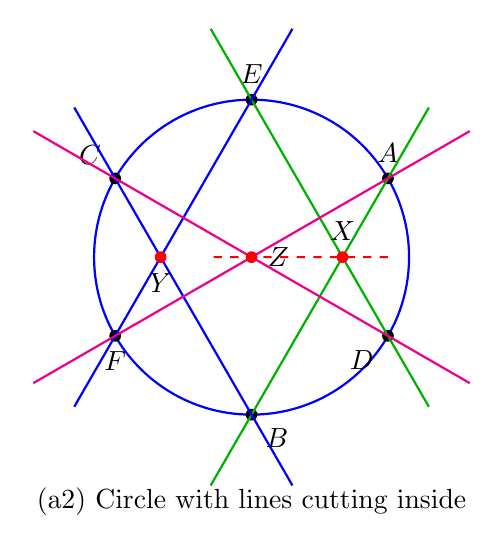
\begin{tikzpicture}[
        point/.style={circle, fill, inner sep=1.5pt},
        scale=0.8
    ]
        % Circle
        \draw[thick, blue] (0,0) circle (2.5cm);
        
        % Points on circle in order around circle: A -> E -> C -> F -> B -> D -> A
        % Hexagon order for Pascal's theorem: A-B-C-D-E-F
        % This arrangement ensures intersections X, Y, Z are inside the circle
        % Spacing: 60° apart (360°/6)
        \node[point, label=above:$A$] (A) at (30:2.5) {};   % First: 30°
        \node[point, label=above:$E$] (E) at (90:2.5) {};   % Second: 90° (upper)
        \node[point, label=above left:$C$] (C) at (150:2.5) {};  % Third: 150° (upper)
        \node[point, label=below:$F$] (F) at (210:2.5) {};  % Fourth: 210° (lower)
        \node[point, label=below right:$B$] (B) at (270:2.5) {};  % Fifth: 270° (lower)
        \node[point, label=below left:$D$] (D) at (330:2.5) {};  % Sixth: 330° (lower)
        
        % Hexagon sides according to Pascal's theorem:
        % X = (AB) ∩ (DE), Y = (BC) ∩ (EF), Z = (CD) ∩ (FA)
        % Extended slightly so intersections are clearly visible inside the circle
        \draw[green!70!black, thick, name path=AB] ($(A)!-0.3!(B)$) -- ($(A)!1.3!(B)$);
        \draw[green!70!black, thick, name path=DE] ($(D)!-0.3!(E)$) -- ($(D)!1.3!(E)$);
        
        \draw[blue, thick, name path=BC] ($(B)!-0.3!(C)$) -- ($(B)!1.3!(C)$);
        \draw[blue, thick, name path=EF] ($(E)!-0.3!(F)$) -- ($(E)!1.3!(F)$);
        
        \draw[magenta, thick, name path=CD] ($(C)!-0.3!(D)$) -- ($(C)!1.3!(D)$);
        \draw[magenta, thick, name path=FA] ($(F)!-0.3!(A)$) -- ($(F)!1.3!(A)$);
        
        % Find intersections according to Pascal's theorem
        \path[name intersections={of=AB and DE, by=X}];
        \path[name intersections={of=BC and EF, by=Y}];
        \path[name intersections={of=CD and FA, by=Z}];
        
        % Draw and label intersection points (X = AB∩DE, Y = BC∩EF, Z = CD∩FA)
        \node[point, fill=red, label=above:$X$] at (X) {};
        \node[point, fill=red, label=below:$Y$] at (Y) {};
        \node[point, fill=red, label=right:$Z$] at (Z) {};
        
        % Draw Pascal line
        \draw[red, dashed, thick] ($(X)!-0.5!(Z)$) -- ($(X)!1.5!(Z)$);
        
        \node[below] at (0, -3.5) {(a2) Circle with lines cutting inside};
    \end{tikzpicture}
    \caption{Pascal's Theorem for a circle: (a1) when lines extend outside the circle, (a2) when lines intersect inside the circle. The intersection points are defined as $X = (AB) \cap (DE)$, $Y = (BC) \cap (EF)$, and $Z = (CD) \cap (FA)$. The red dashed line is the Pascal line.}
\end{figure}

\subsection{Formation of Conic Sections}

Conic sections are curves formed by the intersection of a plane with a double cone (two cones joined at their apex). The type of conic section depends on the angle at which the plane intersects the cone.

\begin{figure}[h!]
    \centering
    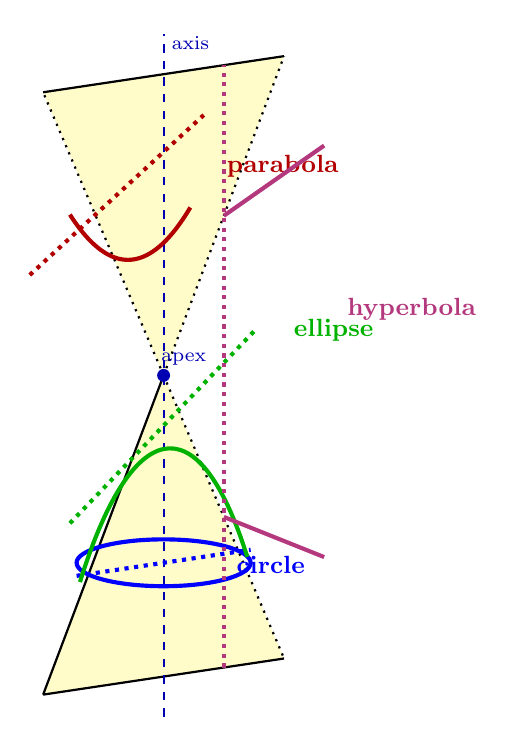
\begin{tikzpicture}[
        scale=0.85,
        every node/.style={font=\small},
        % Improved viewing angle with slight rotation for better 3D perspective
        x={(1cm,0.15cm)},
        y={(0cm,1cm)}
    ]
        % Define cone parameters
        \def\coneHeight{4.5}
        \def\coneRadius{1.8}
        \def\apexY{0}
        
        % Define cone edge coordinates for intersection calculations
        \coordinate (apex) at (0, \apexY);
        \coordinate (upperLeft) at (-\coneRadius, \apexY + \coneHeight);
        \coordinate (upperRight) at (\coneRadius, \apexY + \coneHeight);
        \coordinate (lowerLeft) at (-\coneRadius, \apexY - \coneHeight);
        \coordinate (lowerRight) at (\coneRadius, \apexY - \coneHeight);
        
        % Draw double cone with dotted edges where planes cut through
        % Upper cone - fill first
        \fill[fill=yellow!30, opacity=0.7] 
            (apex) -- (upperLeft) -- (upperRight) -- cycle;
        % Lower cone - fill first
        \fill[fill=yellow!30, opacity=0.7] 
            (apex) -- (lowerLeft) -- (lowerRight) -- cycle;
        
        % Draw cone edges - solid for non-intersected parts, dotted where cut
        % Left edge of upper cone (cut by parabola plane)
        \draw[black, thick, dotted] (apex) -- (upperLeft);
        \draw[black, thick] (apex) -- (lowerLeft);
        % Right edge of upper cone (cut by hyperbola plane)
        \draw[black, thick, dotted] (apex) -- (upperRight);
        % Right edge of lower cone (cut by ellipse and hyperbola planes)
        \draw[black, thick, dotted] (apex) -- (lowerRight);
        % Base edges
        \draw[black, thick] (upperLeft) -- (upperRight);
        \draw[black, thick] (lowerLeft) -- (lowerRight);
        
        % Draw axis
        \draw[dashed, blue!70!black, thick] (0, \apexY - \coneHeight - 0.6) -- (0, \apexY + \coneHeight + 0.6);
        \node[blue!70!black, font=\scriptsize] at (0.4, \apexY + \coneHeight + 0.4) {axis};
        \node[blue!70!black, font=\scriptsize] at (0.3, \apexY + 0.2) {apex};
        \filldraw[blue!70!black] (apex) circle (2.5pt);
        
        % Circle: horizontal plane (perpendicular to axis)
        % Plane line (dotted)
        \draw[dotted, thick, blue, line width=1.5pt] (-1.3, \apexY - 2.8) -- (1.3, \apexY - 2.8);
        % Circle section (intersects cone at x = ±1.3 at y = -2.8)
        \draw[thick, blue, line width=1.5pt] (0, \apexY - 2.8) ellipse (1.3cm and 0.35cm);
        \node[blue, below, font=\small] at (1.6, \apexY - 2.8) {\textbf{circle}};
        
        % Ellipse: angled plane (not parallel to base, not through apex)
        % Plane line (dotted) - angled plane cutting through lower cone
        \draw[dotted, thick, green!70!black, line width=1.5pt] 
            (-1.4, \apexY - 2.0) -- (1.4, \apexY + 0.5);
        % Ellipse section - properly cutting through the cone
        % The ellipse is formed by the intersection of the angled plane with the cone
        % It should appear as an elongated oval cutting through the lower cone
        \draw[thick, green!70!black, line width=1.5pt] 
            (-1.25, \apexY - 2.9) .. controls (-0.5, \apexY - 0.6) and (0.5, \apexY - 0.4) .. (1.25, \apexY - 2.9);
        \node[green!70!black, right, font=\small] at (1.8, \apexY + 0.4) {\textbf{ellipse}};
        
        % Parabola: plane parallel to one side of cone
        % Plane line (dotted) - approximately parallel to left edge
        \draw[dotted, thick, red!70!black, line width=1.5pt] (-2.0, \apexY + 1.8) -- (0.6, \apexY + 3.8);
        % Parabola curve - starts from left edge of upper cone
        % Left edge: from apex to upperLeft, equation y = 4.5/1.8 * x = 2.5x (for x<0)
        % Plane line: y = 1.8 + (3.8-1.8)/(0.6-(-2.0)) * (x-(-2.0)) = 1.8 + 2.0/2.6 * (x+2.0)
        % Intersection: 2.5*x = 1.8 + 0.769*(x+2.0) => x ≈ -1.4, y ≈ -3.5
        \coordinate (parabolaStart) at (-1.4, \apexY - 3.5);
        \draw[thick, red!70!black, line width=1.5pt, domain=-1.4:0.4, samples=100] 
            plot (\x, {\apexY + 1.8 + 0.9*(\x + 0.45)^2});
        \node[red!70!black, right, font=\small] at (0.8, \apexY + 3.0) {\textbf{parabola}};
        
        % Hyperbola: vertical plane cutting both cones
        % Plane line (dotted) - vertical at x = 0.9
        \draw[dotted, thick, magenta!70!black, line width=1.5pt] 
            (0.9, \apexY - \coneHeight) -- (0.9, \apexY + \coneHeight);
        % Intersection points with cone edges
        % Right edge of upper cone: from apex to upperRight
        % Line from (0,0) to (1.8, 4.5): y = 4.5/1.8 * x = 2.5*x
        % At x=0.9: y = 2.25
        % Right edge of lower cone: from apex to lowerRight
        % Line from (0,0) to (1.8, -4.5): y = -4.5/1.8 * x = -2.5*x
        % At x=0.9: y = -2.25
        \coordinate (hyperbolaUpper) at (0.9, \apexY + 2.25);
        \coordinate (hyperbolaLower) at (0.9, \apexY - 2.25);
        % Upper branch (right side) - starts from upper intersection point
        \draw[thick, magenta!70!black, line width=1.5pt, domain=0.9:2.4, samples=100] 
            plot (\x, {\apexY + 2.25 + 0.55*sqrt((\x - 0.9)^2)});
        % Lower branch (right side) - starts from lower intersection point
        \draw[thick, magenta!70!black, line width=1.5pt, domain=0.9:2.4, samples=100] 
            plot (\x, {\apexY - 2.25 - 0.55*sqrt((\x - 0.9)^2)});
        \node[magenta!70!black, right, font=\small] at (2.6, \apexY + 0.6) {\textbf{hyperbola}};
        
    \end{tikzpicture}
    \caption{Formation of conic sections by intersecting a double cone with planes at different angles. A \textbf{circle} is formed by a horizontal plane (perpendicular to the axis), an \textbf{ellipse} by an angled plane (not parallel to the base and not through the apex), a \textbf{parabola} by a plane parallel to one side of the cone, and a \textbf{hyperbola} by a vertical plane cutting both cones.}
\end{figure}

\subsection{High-Level Proof of Pascal's Theorem}

A complete proof of Pascal's Theorem requires advanced techniques from algebraic geometry or projective geometry. Here we outline the main ideas:

\subsubsection{Projective Geometry Framework}

We work in the projective plane, where:
\begin{itemize}
    \item Every two distinct lines intersect (parallel lines meet at infinity)
    \item All conics are projectively equivalent
    \item The theorem can be stated purely in terms of incidence relations
\end{itemize}

\subsubsection{Key Steps}

\begin{enumerate}
    \item \textbf{Projective Equivalence}: Since all conics are projectively equivalent, it suffices to prove the theorem for one conic (e.g., a circle).
    
    \item \textbf{Coordinate Geometry Approach}: Using homogeneous coordinates, we can express the condition that six points lie on a conic as a determinant condition. The collinearity of $X, Y, Z$ can then be verified algebraically.
    
    \item \textbf{Bezout's Theorem}: This fundamental result in algebraic geometry states that two curves of degrees $m$ and $n$ intersect in at most $mn$ points (counting multiplicity). This helps control the intersection structure.
    
    \item \textbf{Cayley-Bacharach Theorem}: A more general result that implies Pascal's Theorem as a special case. It states that if two cubic curves intersect in nine points, then any cubic through eight of them must pass through the ninth.
\end{enumerate}

\subsubsection{The Elegant Insight}

The most elegant modern proof uses the theory of cubic curves. The six points on the conic, together with the three intersection points $X, Y, Z$, can be related through cubic curves. The fact that the six points lie on a conic (a quadratic curve) forces a relationship that implies $X, Y, Z$ are collinear.

\subsubsection{Connection to Pappus}

As we've seen, Pappus's hexagon theorem is the special case where the conic degenerates to two lines. This demonstrates the power of projective geometry: by working in the projective plane and considering degenerate cases, we unify many seemingly different theorems.

\section{Future Works and Open Problems}

Pappus's hexagon theorem opens many exciting doors for further exploration. Here are some directions that students and enthusiasts can pursue:

\begin{enumerate}
    \item \textbf{Exploring Other Theorems}: Pappus's hexagon theorem is closely related to other beautiful results in projective geometry, such as Desargues's Theorem and Pascal's Theorem. Try to understand these connections and see how they form a unified picture of projective geometry. These theorems often appear together in olympiad problems!
    
    \item \textbf{Algebraic Approaches}: While we've presented geometric and projective proofs, you can explore purely algebraic proofs using coordinate geometry. Try setting up coordinates for the points and lines, then verify the collinearity of $X$, $Y$, and $Z$ using algebra. This approach helps develop computational skills and provides a different perspective on the theorem.
    
    \item \textbf{Constructive Proofs and Algorithms}: Can you develop a step-by-step algorithm that, given the points $A, B, C$ on line $g$ and $a, b, c$ on line $h$, computes the Pappus line? This is a great programming exercise that combines geometry with computation. You could even create an interactive visualization!
    
    \item \textbf{Applications in Computer Graphics}: Projective geometry, including Pappus's hexagon theorem, has practical applications in computer vision and 3D graphics. Understanding how cameras work, how to calibrate them, and how to reconstruct 3D scenes from 2D images all use projective geometry. This is a beautiful example of how pure mathematics connects to real-world technology.
    
    \item \textbf{Generalizations and Patterns}: What happens if you have more points on each line? Can you find patterns or generalizations? Try experimenting with different configurations and see what properties remain true. This kind of exploration is at the heart of mathematical discovery.
    
    \item \textbf{Special Cases and Constructions}: Explore special cases like when the lines are parallel, perpendicular, or when certain points coincide. Try to construct the Pappus line using only a straightedge (ruler without markings)---this connects to classical geometric constructions.
\end{enumerate}

These directions show that Pappus's hexagon theorem is not just a single result, but a gateway to deeper understanding of geometry, algebra, and their beautiful interconnections. Whether you're interested in pure mathematics, computer science, or applications, there's something here to explore!

\section{Conclusions}

Pappus's hexagon theorem stands as a cornerstone of projective geometry, connecting classical Euclidean geometry to modern algebraic geometry. We have seen:

\begin{itemize}
    \item The theorem's elegant statement about collinearity of intersection points
    \item Its historical significance dating back to Pappus of Alexandria
    \item Two proof approaches: the computational affine transformation method and the elegant connection to Pascal's Theorem
    \item The deep relationship between Pappus's hexagon theorem and Pascal's Theorem through the concept of degenerate conics
    \item The power of projective geometry in unifying seemingly different geometric phenomena
\end{itemize}

The theorem demonstrates that sometimes the most elegant proofs come from recognizing that a specific result is a special case of a more general theorem. By viewing two lines as a degenerate conic, Pappus's hexagon theorem becomes an immediate consequence of Pascal's Theorem, revealing the beautiful structure underlying projective geometry.

For olympiad students, mastering Pappus's hexagon theorem provides:
\begin{itemize}
    \item A deeper understanding of projective geometry
    \item Experience with transformation techniques (affine transformations)
    \item Insight into how degenerate cases can illuminate general theorems
    \item A gateway to more advanced topics in algebraic geometry
\end{itemize}

\vspace{2em}
\noindent
\textbf{Contact Information:}\\[0.5em]
LinkedIn: \href{https://www.linkedin.com/in/nguyenvuhung/}{https://www.linkedin.com/in/nguyenvuhung/}\\[0.3em]
GitHub: \href{https://github.com/vuhung16au/}{https://github.com/vuhung16au/}\\[0.3em]
Repository: \href{https://github.com/vuhung16au/math-olympiad-ml/tree/main/PappusTheorem}{https://github.com/vuhung16au/math-olympiad-ml/tree/main/PappusTheorem}

\end{document}
